
% ===========================
\chapter{Grundlagen}
\label{grundlagen}
% ===========================

In diesem Kapitel werden die zum Verständnis nötigen Grundlagen für diese Arbeit erklärt. Dabei wird im Abschnitt \ref{grundlagen_fahren} der Stand der Technik von automatisierten Fahrfunktionen und deren Entwicklung beschrieben. Im Abschnitt \ref{grundlagen_nn} wird maschinelles Lernen im Allgemeinen und im Speziellen künstliche neuronale Netze, die für die Umsetzung dieser Arbeit nötig sind, beschrieben.


% ===========================
\section{Hochautomatisiertes Fahren}
\label{grundlagen_fahren}
% ===========================

Hochautomatisiertes Fahren wird in den vergangenen Jahren zunehmend von der Automobilindustrie vorangetrieben. Aktuelle \gls{fas} wie der Spurhalteassistant oder die Abstandsregelung sind nach der Norm SAE J3016 (Abbildung \ref{fig_level_autonomes_fahren}) bei Level 2 des autonomen Fahrens eingeordnet. Mit neuen Technologien werden immer mehr Funktionen für automatisiertes Fahren entwickelt und verknüpft. Es entstehen zunehmend komplexe Fahrfunktionen mit einer steigenden Anzahl möglicher Fahrsituationen und Szenarien \cite{king2017identification}. Das stellt Automobilhersteller und Automobilzulieferer vor eine große Herausforderung, da die Systemkomplexität wächst. Das schließt sowohl die Entwicklung von \gls{fas} als auch die dazu benötigten Testszenarien ein \cite{pfeffer2016continuous}.

In den folgenden Abschnitten wird erläutert wie aktuell diesen Herausforderungen begegnet wird. In Abschnitt \ref{grundlagen_fahren_entwicklung} wird ein allgemeiner Überblick über die aktuellen Entwicklungsmethodiken für \gls{fas} gegeben. Danach werden in Abschnitt \ref{grundlagen_fahren_szenarien} bisherige Ansätze für die Klassifizierung von Fahrszenarien vorgestellt.

\begin{figure}[h]
\centering
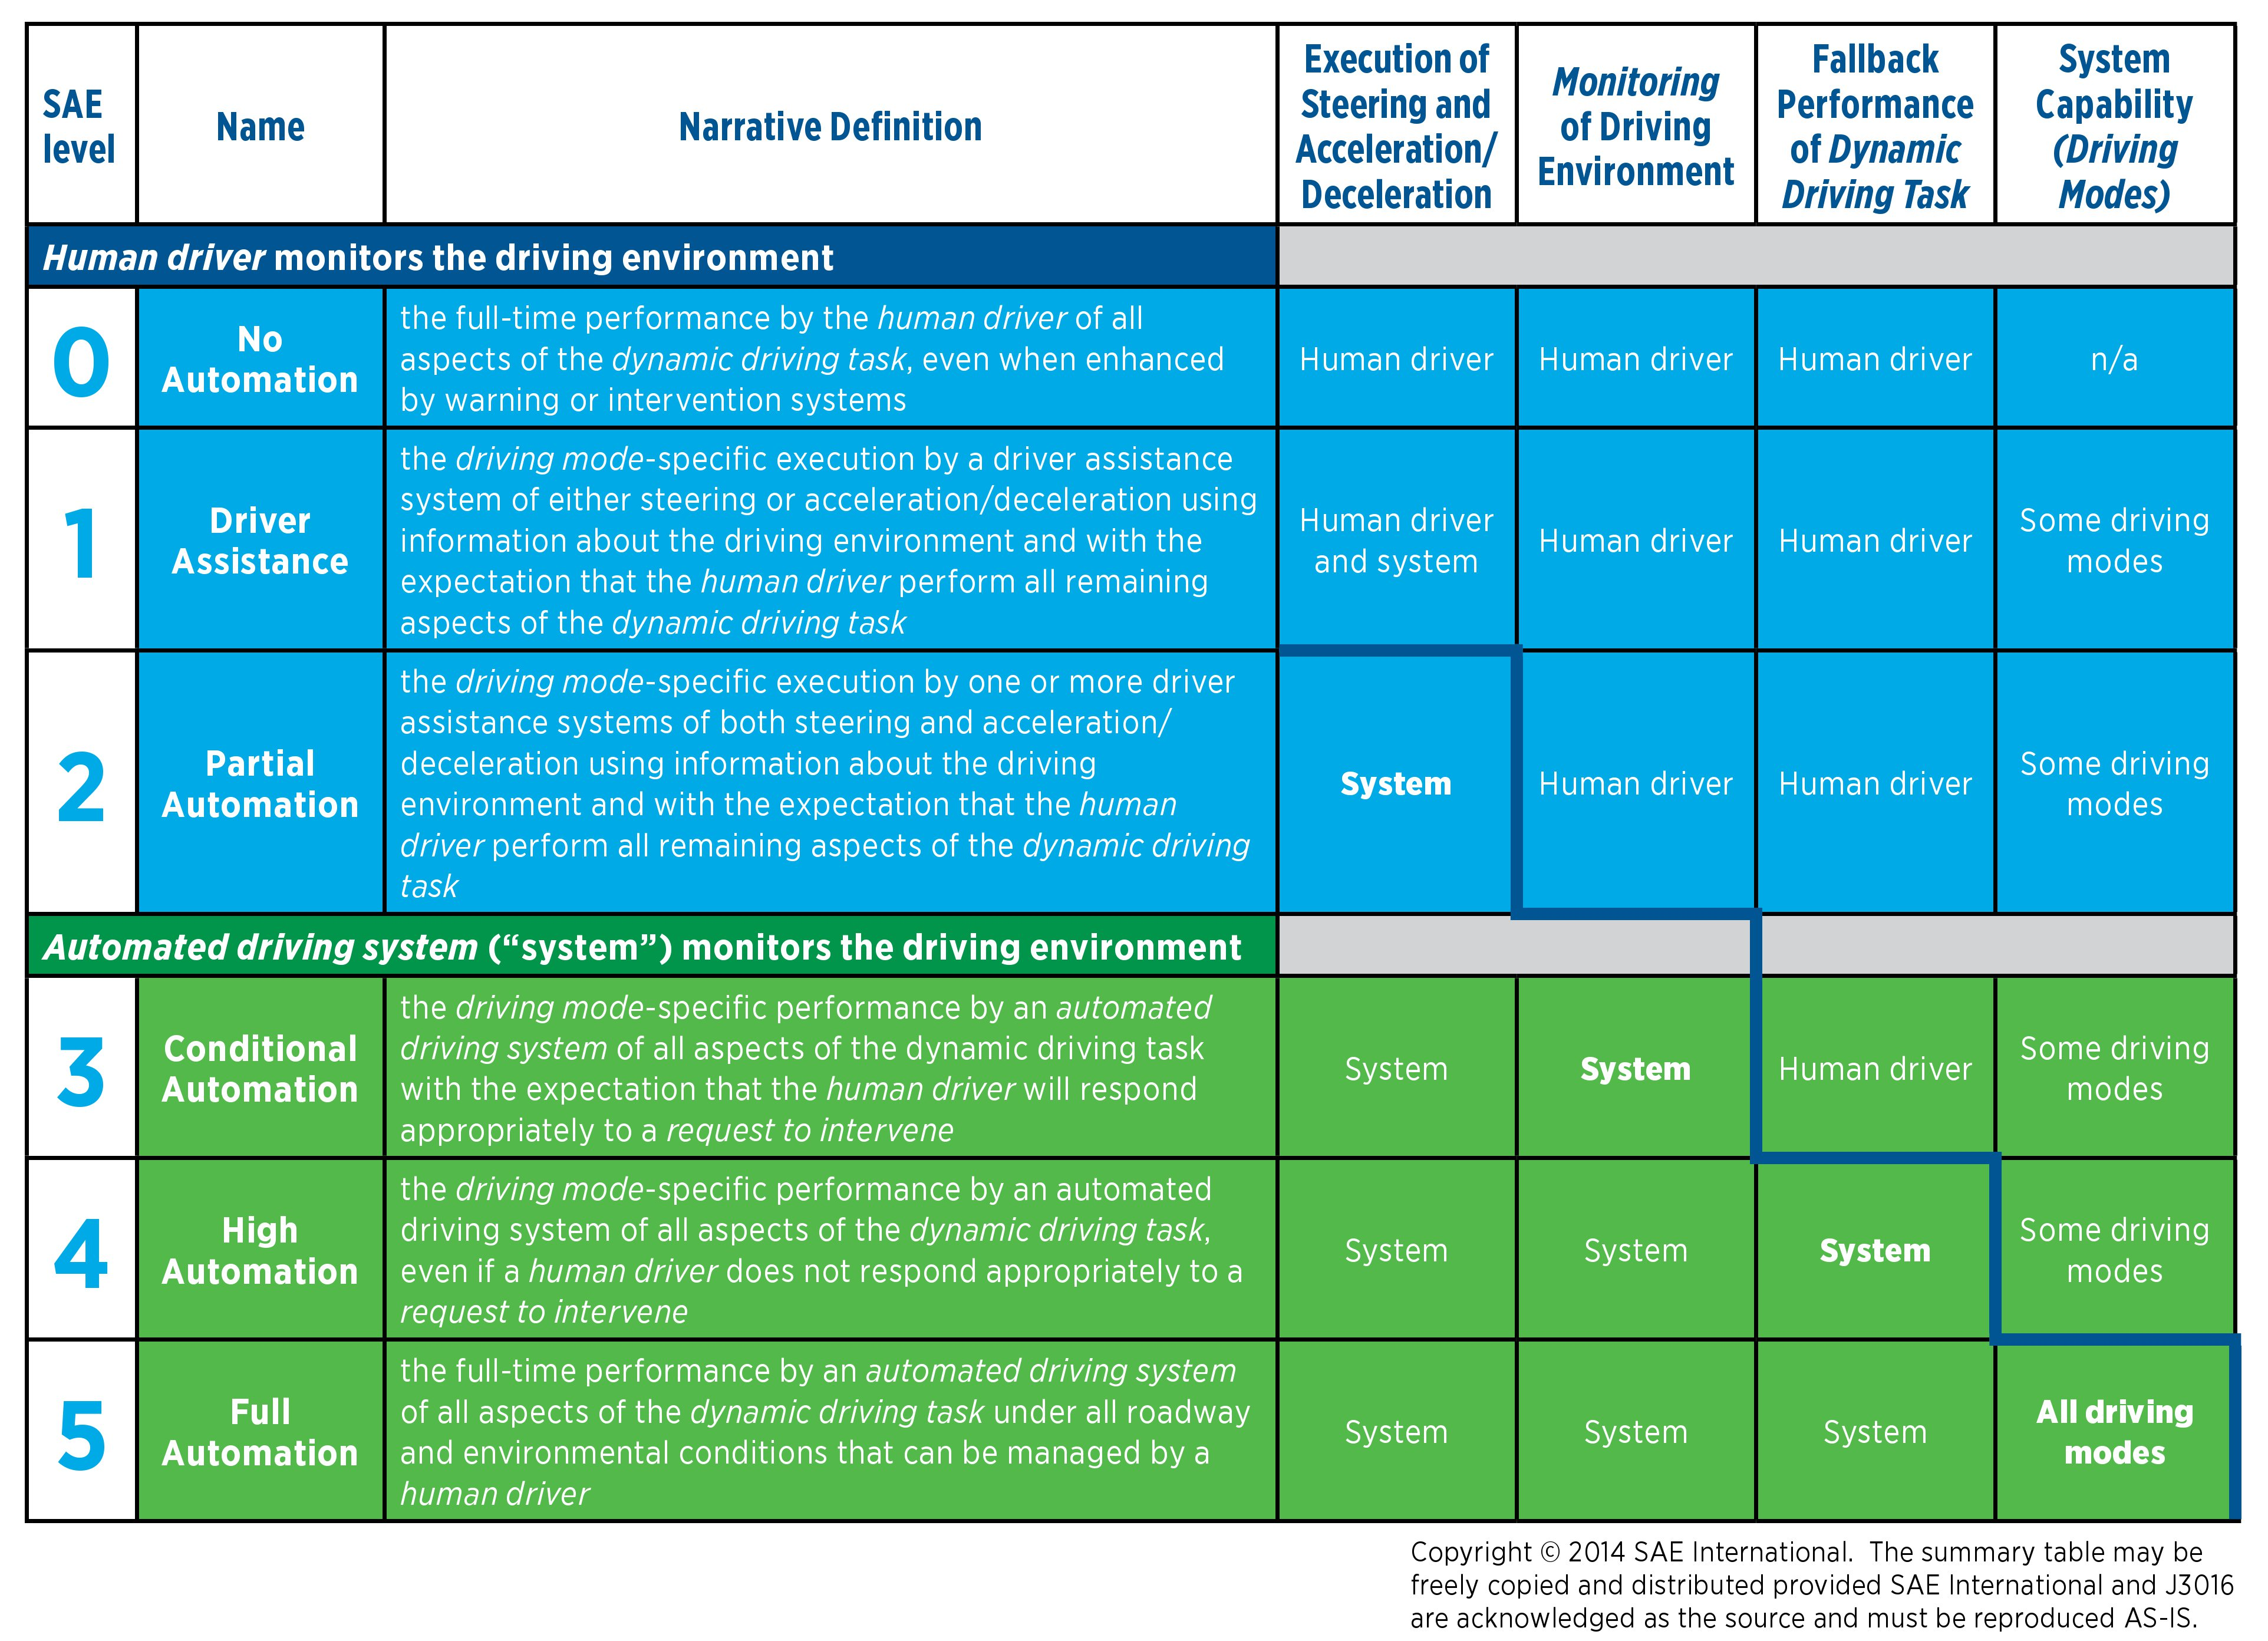
\includegraphics[scale=0.7]{level_autonomes_fahren.jpg}
\caption{Norm SAE J3016 für die Level des autonomen Fahrens, entnommen aus \cite{sae2014taxonomy}}
\label{fig_level_autonomes_fahren}
\end{figure}


% ===========================
\subsection{Entwicklung von Fahrerassistenzfunktionen}
\label{grundlagen_fahren_entwicklung}
% ===========================

\gls{fas} sind Funktionen im Kraftfahrzeug, die den Fahrer unterstützen. Diese Systeme nutzen Sensordaten, wie Radar-, Ultraschall-, oder Kameradaten, aus dem Fahrzeug um den Fahrer dann auf Basis der abgeleiteten Informationen zu unterstützen. Beispielsweise erkennt ein Spurhalteassistent wenn das Fahrzeug die Spur verlässt und kann die Fahrlinie korrigieren. 

\gls{fas} werden in der Automobilindustrie mit dem V-Modell entwickelt. Das V-Modell ist ein chronologischer Entwicklungsprozess und aus der Softwareentwicklung adaptiert \cite{vmodell2005}. Das V-Modell kann in einen linken absteigenden und einen rechten aufsteigenden Ast unterteilt werden. Der linke Ast enthält die Funktionsanforderungen, die nach unten weiter detailliert und aufgeschlüsselt werden. Der rechte Ast umfasst aufsteigend Funktionstests auf dem jeweiligen Detaillierungsgrad \cite{hakuli2015virtuelle}. Das V-Modell ist schematisch in Abbildung \ref{fig_v_modell} dargestellt.

\begin{figure}[h]
\centering
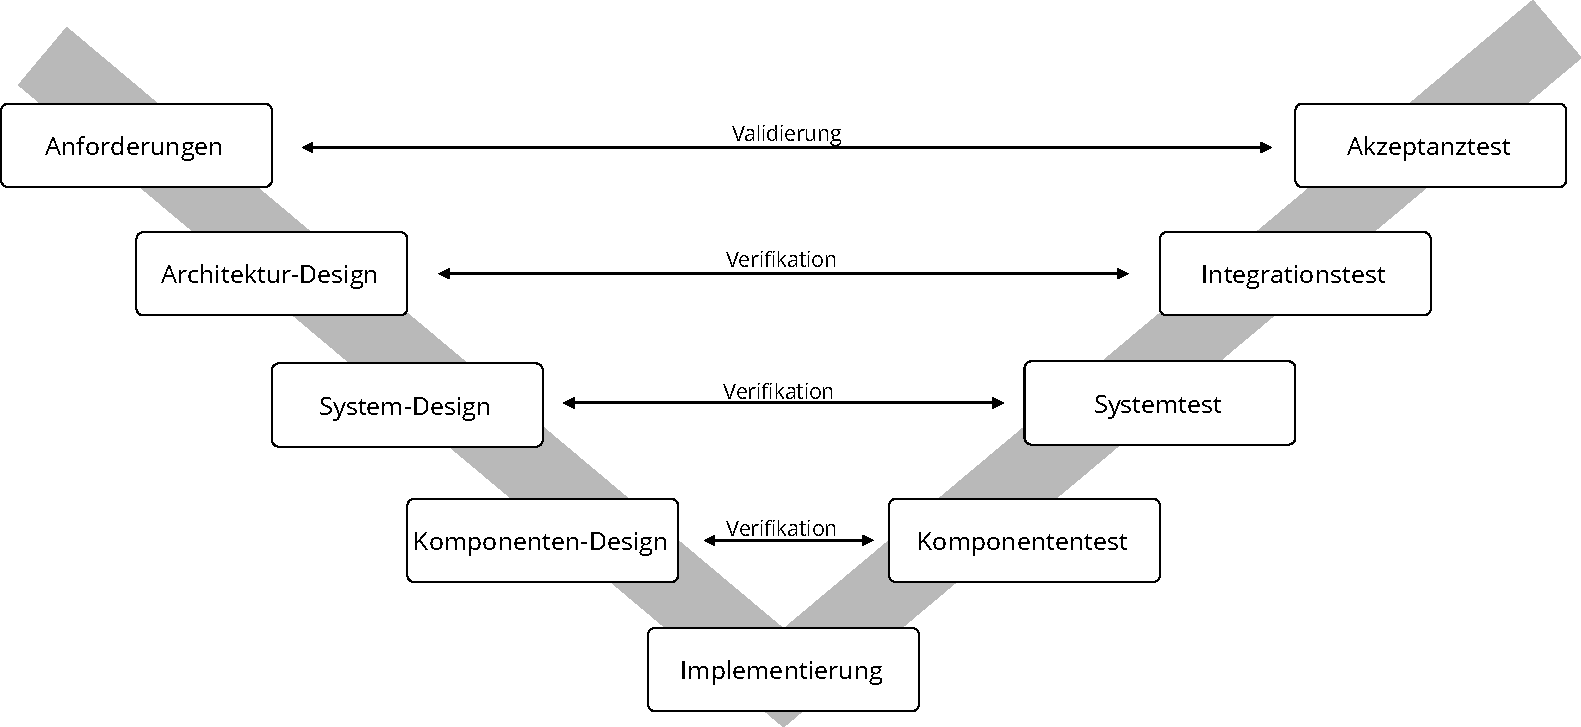
\includegraphics[scale=0.5]{v_modell.pdf}
\caption{V-Modell, adaptiert von \cite{hakuli2015virtuelle}}
\label{fig_v_modell}
\end{figure}

Die Schritte auf dem absteigenden und aufsteigenden Ast haben jeweils eine Beziehung. Jeder Test auf dem aufsteigenden Ast verifiziert bzw. validiert den dazugehörigen Entwicklungsschritt auf dem absteigenden Ast. Demenstsprechend werden oben im V-Modell die Kundenanforderungen auf dem absteigenden Ast erfasst und auf dem aufsteigenden Ast validiert. Unten im V-Modell werden einzelne Hardware- oder Softwarekomponenten entwickelt, die die entsprechenden Kundenanforderungen von oben lösen sollen, und auf dem aufsteigenden Ast verifiziert \cite{hakuli2015virtuelle}.

Die Validierung und Verifikation von \gls{fas} folgt dem Testkonzept. Ein Testkonzept umfasst die Analyse des Testobjektes, die Generierung von Testfällen, die Durchführung von Tests und schließlich die Testauswertung \cite{schuldt2013effiziente}.

\begin{figure}[h]
\centering
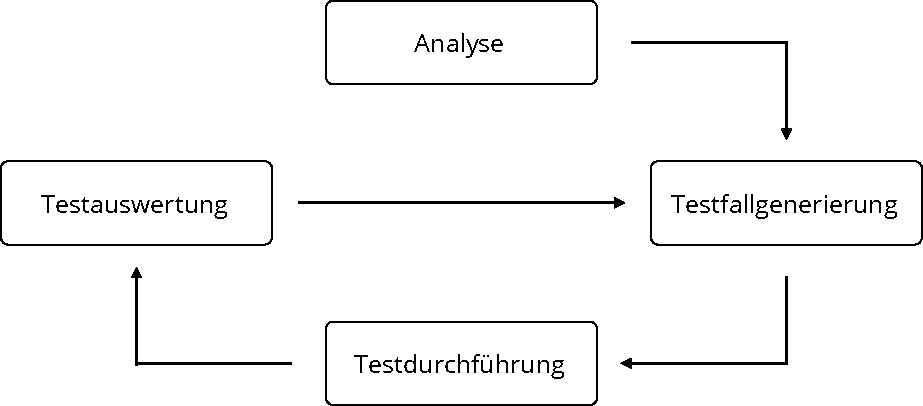
\includegraphics[scale=0.5]{testfallerstellung.pdf}
\caption{Testfallerstellung, von \cite{schuldt2013effiziente}}
\label{fig_testfallerstellung}
\end{figure}

Testfälle werden bereits möglichst früh im Entwicklungsprozess erstellt um die Qualität von \gls{fas} und einzelnen Komponenten möglichst hoch zu halten \cite{wachenfeld2015freigabe}. Hierfür werden in der Praxis virtuelle Fahrversuche eingesetzt. Die Idee ist eine stufenweise Digitalisierung von Komponenten aus dem realen Fahrversuch mit den Zielen die Reproduzierbarkeit zu steigern, den Aufwand zu reduzieren und insgesamt flexibler zu werden. Im virtuellen Fahrversuch werden in der frühen Konzeptphase alle Komponenten virtuell getestet und dann schrittweise durch Hardwarekomponenten ersetzt. Schließlich werden alle Komponenten im realen Fahrversuch auf der Straße mit realem Fahrer und anderen Verkehrsteilnehmern getestet \cite{hakuli2015virtuelle}.

Beim virtuellen Fahrversuch spielen die Konzepte \gls{mil}, \gls{sil}, \gls{hil} und \gls{vil} eine wichtige Rolle. Mit \gls{mil} und \gls{sil} werden Funktionen auf Basis von Simulationsmodellen getestet \cite{berg2015vehicle}. Dabei werden Hardwarekomponenten simuliert. Mit fortschreitender Entwicklung werden immer mehr Simulationskomponenten durch die entsprechende Hardware ersetzt und mit \gls{hil} getestet \cite{hakuli2015virtuelle}. \gls{vil} schließt schließlich die Lücke zwischen virtuellem Fahrversuch und realem Fahrversuch. Dieses Testkonzept macht die Komplexität bei der Entwicklung von \gls{fas} beherrschbar und reduziert den Testaufwand \cite{schwab2014durchgangige}. Für die Freigabe von \gls{fas} ist die Realfahrt aber die wichtigste Methode, da sie aktuell die beste Validierung bei annehmbaren ökonomischen Aufwand ist \cite{wachenfeld2015freigabe}.

Mit steigender Automatisierung von \gls{fas} steigt auch die Anzahl möglicher Situationen und damit die Anzahl der benötigten Testfälle. Testfälle müssen alle potentiell möglichen Situationen, in denen das \gls{fas} zum Einsatz kommen kann, abdecken. Dadurch steigt mit hochautomatisierten Funktionen der Aufwand für Testfallgenerierung und -durchführung ins Unüberschaubare. Eine Möglichkeit für die Reduzierung von Testfällen ist es kritische Situationen zu finden und Testfälle mit weniger kritischen Situationen zu entfernen \cite{wachenfeld2015freigabe}.





heute schon mehrere Millionen Testkilometer für die 
Bei der Validierung und Verifikation von aktuellen \gls{fas} werden heute schon mehrere Millionen Testkilometer benötigt \cite{wachenfeld2015freigabe}. 





Therefore, approaches for the evaluation of the entire test drive are required. Additionally, the recognition of driving scenarios and maneuvers of the vehicle is highly important for the activation of appropriate assessments within a test drive. \cite{otten2018automated}



% ===========================
\subsection{Klassifizierung von Fahrszenarien}
\label{grundlagen_fahren_szenarien}
% ===========================

- Terminologie, Unterschiedung Szene, Szenario, ...
- Tabelle + Erklärung

Duis autem vel eum iriure dolor in hendrerit in vulputate velit esse molestie consequat, vel illum dolore eu feugiat nulla facilisis at vero eros et accumsan et iusto odio dignissim qui blandit praesent luptatum zzril delenit augue duis dolore te feugait nulla facilisi.   


% ===========================
\section{Künstliche Neuronale Netze}
\label{grundlagen_nn}
% ===========================

Duis autem vel eum iriure dolor in hendrerit in vulputate velit esse molestie consequat, vel illum dolore eu feugiat nulla facilisis.


% ===========================
\subsection{Maschinelles Lernen}
\label{grundlagen_nn_ml}
% ===========================

Duis autem vel eum iriure dolor in hendrerit in vulputate velit esse molestie consequat, vel illum dolore eu feugiat nulla facilisis at vero eros et accumsan et iusto odio dignissim qui blandit praesent luptatum zzril delenit augue duis dolore te feugait nulla facilisi. 


% ===========================
\subsection{Convolutional Neural Network}
\label{grundlagen_nn_cnn}
% ===========================


\begin{table}[h]
\centering
\begin{tabular}{l | l | l}
A & B & C \\
\hline
1 & 2 & 3 \\
4 & 5 & 6
\end{tabular}
\caption{very basic table}
\label{tab:abc}
\end{table}


% ===========================
\subsection{Recurrent Neural Network}
\label{grundlagen_nn_rnn}
% ===========================

Lorem ipsum dolor sit amet, consectetuer adipiscing elit, sed diam nonummy nibh euismod tincidunt ut laoreet dolore magna aliquam erat volutpat \cite{latexcompanion}. 


% ===========================
\subsection{Training mit synthetischen Daten}
\label{grundlagen_nn_synthetisch}
% ===========================

Lorem ipsum dolor sit amet, consectetuer adipiscing elit, sed diam nonummy nibh euismod tincidunt ut laoreet dolore magna aliquam erat volutpat \cite{latexcompanion}. 


